%=================================================================
% CSE 4345 — Big Data Analytics
% Week 1, Part 1: Digital Data Landscape & Introduction to Big Data
% Department of CSE, Premier University
% Part 1 covers: Introduction · Core Concepts · Ivy League Alignment
%               · Student Assessment · Textbook References
% Part 2 covers: Seminal Research (Laney 2001) · Case Study (McKinsey 2011)
%=================================================================

\documentclass[aspectratio=169,10pt]{beamer}

%---------- Packages ----------
\usepackage[utf8]{inputenc}
\usepackage[T1]{fontenc}
\usepackage{booktabs}
\usepackage{xcolor}
\usepackage{tikz}
\usetikzlibrary{shapes.geometric, positioning, arrows.meta}
\usepackage{amsmath}
\usepackage{graphicx}
\usepackage{multicol}
\usepackage{enumerate}    % for (a)(b)(c) in MCQ

%---------- Theme ----------
\usetheme{Madrid}

%---------- Premier University Color Identity ----------
\definecolor{PUNavy}{RGB}{10,36,99}
\definecolor{PUGold}{RGB}{197,151,37}
\definecolor{PULightBlue}{RGB}{210,228,255}
\definecolor{PUTeal}{RGB}{0,100,100}
\definecolor{PUGray}{RGB}{90,90,90}

\setbeamercolor{palette primary}{bg=PUNavy, fg=white}
\setbeamercolor{palette secondary}{bg=PUNavy!85, fg=white}
\setbeamercolor{palette tertiary}{bg=PUNavy!70, fg=white}
\setbeamercolor{palette quaternary}{bg=PUNavy, fg=white}
\setbeamercolor{structure}{fg=PUNavy}
\setbeamercolor{title}{bg=PUNavy, fg=PUGold}
\setbeamercolor{subtitle}{fg=white}
\setbeamercolor{frametitle}{bg=PUNavy, fg=PUGold}
\setbeamercolor{alerted text}{fg=PUGold!85!black}
\setbeamercolor{block title}{bg=PUNavy, fg=white}
\setbeamercolor{block body}{bg=PULightBlue!45}
\setbeamercolor{block title alerted}{bg=PUGold!80!black, fg=white}
\setbeamercolor{block body alerted}{bg=PUGold!12}
\setbeamercolor{block title example}{bg=PUTeal, fg=white}
\setbeamercolor{block body example}{bg=PUTeal!10}
\setbeamercolor{section in toc}{fg=PUNavy}
\setbeamercolor{itemize item}{fg=PUGold!80!black}
\setbeamercolor{itemize subitem}{fg=PUNavy!70}

\setbeamertemplate{navigation symbols}{}
\setbeamertemplate{itemize item}{\scriptsize\raise1.5pt\hbox{\textbullet}}
\setbeamertemplate{itemize subitem}{\scriptsize\raise1pt\hbox{--}}

%---------- Section slide (mini ToC on section change) ----------
\AtBeginSection[]{
  \begin{frame}[plain]
    \vfill
    \centering
    \begin{beamercolorbox}[sep=12pt,center,shadow=true,rounded=true]{block title}
      \usebeamerfont{title}\insertsectionhead\par
    \end{beamercolorbox}
    \vfill
  \end{frame}
}

%---------- Title metadata ----------
\title[CSE 4345 \textbar{} Week 1, Part 1]{CSE 4345: Big Data Analytics}
\subtitle{Week 1, Part 1 \textemdash\ Digital Data Landscape \& Introduction to Big Data}
\author[Dept.\ of CSE]{Rokan Uddin Faruqui \\ Professor \\ Department of Computer Science \& Engineering\\[4pt]
       \small University of Chittagong, Chittagong}
\institute{}
\date{CSE, PUC, Spring 2026}

%=================================================================
\begin{document}
%=================================================================

%----------------------------------------------------------------
% TITLE SLIDE
%----------------------------------------------------------------
\begin{frame}
  \titlepage
\end{frame}

%----------------------------------------------------------------
% COURSE INFO
%----------------------------------------------------------------
\begin{frame}{Course \& Lecture Information}
  \begin{columns}[T]
    \column{0.47\textwidth}
      \begin{block}{Course Details}
        \begin{tabular}{ll}
          \textbf{Code:}     & CSE 4345 \\
          \textbf{Credits:}  & 3 (Theory) \\
          \textbf{Type:}     & Elective -- Data Science \\
          \textbf{Pre-req:}  & CSE 2221 -- DBMS \\
        \end{tabular}
      \end{block}
      \vspace{6pt}
      \begin{block}{Today}
        \begin{tabular}{ll}
          \textbf{Week / Part:} & 1 of 11 \textbar\ Part 1 of 2 \\
          \textbf{CLO:}   & CLO1 \\
          \textbf{PLO:}   & PLO(a) \\
        \end{tabular}
      \end{block}

    \column{0.50\textwidth}
      \begin{alertblock}{CLO1}
        \textit{``Understand big data characteristics''}
      \end{alertblock}
      \vspace{6pt}
      \begin{exampleblock}{Part 1 Covers}
        \begin{itemize}
          \item The modern data explosion
          \item Types of digital data
          \item The 3Vs and 5Vs framework
          \item Distributed computing basics
          \item Ivy League alignment
          \item Student assessment pool
        \end{itemize}
      \end{exampleblock}
  \end{columns}
\end{frame}

%----------------------------------------------------------------
% AGENDA
%----------------------------------------------------------------
\begin{frame}{Lecture Agenda}
  \tableofcontents
\end{frame}

%================================================================
\section{The Data Revolution}
%================================================================

\begin{frame}{We Are Living in the Data Age}
  \begin{columns}[T]
    \column{0.58\textwidth}
      \textbf{Data generated every 60 seconds (2024 estimates):}
      \vspace{4pt}
      \begin{itemize}
        \item \textbf{6{,}000} tweets posted per second on X (Twitter)
        \item \textbf{500 hours} of video uploaded to YouTube per minute
        \item \textbf{1 million} messages sent on WhatsApp
        \item \textbf{5 million} Google search queries executed
        \item \textbf{500 TB} of new data ingested by Facebook daily
        \item \textbf{50{,}000} apps downloaded from Apple App Store
      \end{itemize}
      \vspace{6pt}
      \begin{alertblock}{IDC Global Datasphere Forecast}
        By 2025, the world will generate and replicate \textbf{175 zettabytes} of data annually\textemdash a 23$\times$ increase from 2018.
      \end{alertblock}

    \column{0.38\textwidth}
      \begin{block}{Data Volume Units}
        \centering
        \small
        \renewcommand{\arraystretch}{1.2}
        \begin{tabular}{lr}
          \toprule
          \textbf{Unit} & \textbf{Bytes} \\
          \midrule
          Kilobyte (KB)  & $10^{3}$ \\
          Megabyte (MB)  & $10^{6}$ \\
          Gigabyte (GB)  & $10^{9}$ \\
          Terabyte (TB)  & $10^{12}$ \\
          Petabyte (PB)  & $10^{15}$ \\
          Exabyte (EB)   & $10^{18}$ \\
          \alert{Zettabyte (ZB)} & \alert{$10^{21}$} \\
          Yottabyte (YB) & $10^{24}$ \\
          \bottomrule
        \end{tabular}
      \end{block}
  \end{columns}
\end{frame}

%----------------------------------------------------------------
\begin{frame}{The Fundamental Problem: Single Machine vs.\ Reality}
  \begin{columns}[T]
    \column{0.52\textwidth}
      \begin{block}{What a Single Server Can Handle (2024)}
        \vspace{2pt}
        \renewcommand{\arraystretch}{1.2}
        \begin{tabular}{ll}
          \toprule
          \textbf{Resource} & \textbf{Maximum} \\
          \midrule
          RAM (high-end server)    & $\sim$64 TB \\
          Disk throughput (SSD)    & $\sim$7 GB/s \\
          RDBMS comfortable limit  & $\sim$10--50 TB \\
          Time to read 1 PB at 7 GB/s & $\approx$41 hours \\
          \bottomrule
        \end{tabular}
      \end{block}
      \vspace{6pt}
      \begin{alertblock}{The Gap}
        Modern organisations generate data at rates that \textbf{fundamentally outpace} what any single machine can store, process, or query in acceptable time.
      \end{alertblock}

    \column{0.45\textwidth}
      \begin{exampleblock}{The Big Data Engineering Response}
        \vspace{2pt}
        \begin{itemize}
          \item \textbf{Distribute} data across hundreds of commodity nodes
          \item \textbf{Move computation to data} rather than fetching data to a central processor
          \item \textbf{Replicate} blocks for fault tolerance (3$\times$ in HDFS)
          \item \textbf{Parallelise} every operation\textemdash divide, compute, merge
        \end{itemize}
        \vspace{4pt}
        \textbf{Core principle (GFS, 2003):}\\
        \textit{``Commodity hardware will fail.  Design for failure from the start.''}
      \end{exampleblock}
  \end{columns}
\end{frame}

%================================================================
\section{Types of Digital Data}
%================================================================

\begin{frame}{Three Categories of Digital Data}
  \begin{center}
  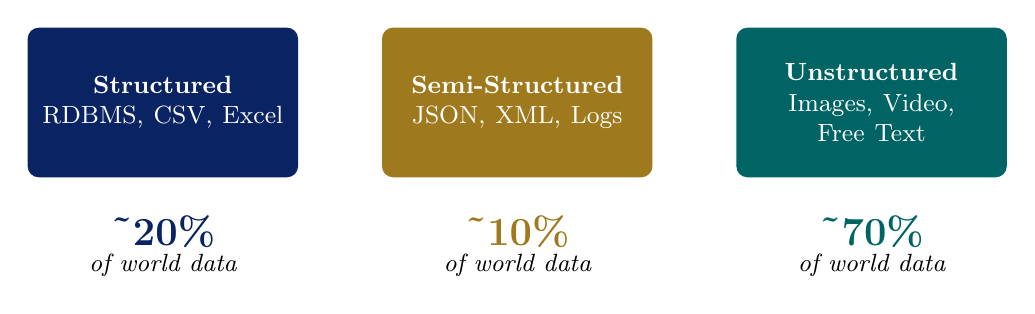
\begin{tikzpicture}[
      box/.style={rectangle, rounded corners=4pt,
                  minimum width=3.4cm, minimum height=1.9cm,
                  text width=3.2cm, align=center, font=\small\bfseries},
      pct/.style={font=\Large\bfseries},
      lbl/.style={font=\small\itshape}
    ]
    % Boxes
    \node[box, fill=PUNavy,        text=white]  (S)  at (0,0)
        {Structured\\\normalfont\small RDBMS, CSV, Excel};
    \node[box, fill=PUGold!80!black, text=white] (SS) at (4.5,0)
        {Semi-Structured\\\normalfont\small JSON, XML, Logs};
    \node[box, fill=PUTeal,          text=white] (U)  at (9,0)
        {Unstructured\\\normalfont\small Images, Video, Free Text};

    % Percentages
    \node[pct, below=0.35cm of S,  text=PUNavy]          {\textasciitilde20\%};
    \node[pct, below=0.35cm of SS, text=PUGold!80!black] {\textasciitilde10\%};
    \node[pct, below=0.35cm of U,  text=PUTeal]          {\textasciitilde70\%};

    \node[lbl, below=0.85cm of S]  {of world data};
    \node[lbl, below=0.85cm of SS] {of world data};
    \node[lbl, below=0.85cm of U]  {of world data};
  \end{tikzpicture}
  \end{center}
  \vspace{6pt}
  \begin{alertblock}{Key Insight}
    Over \textbf{80\%} of the world's data is unstructured\textemdash this is the frontier that Big Data tools are built to unlock.  Traditional SQL databases cannot process it without significant pre-processing.
  \end{alertblock}
\end{frame}

%----------------------------------------------------------------
\begin{frame}{Structured Data}
  \begin{columns}[T]
    \column{0.52\textwidth}
      \begin{block}{Definition}
        Data organised into a \textbf{predefined schema} (rows and columns).  Schema is enforced \emph{at write time} (\textbf{schema-on-write}).
      \end{block}
      \vspace{4pt}
      \textbf{Characteristics:}
      \begin{itemize}
        \item Fixed, known schema before ingestion
        \item Stored in relational databases (MySQL, Oracle, PostgreSQL)
        \item Queryable directly with standard SQL
        \item Strong ACID guarantees
        \item Easy to index, filter, aggregate
      \end{itemize}
      % \vspace{4pt}
      % \begin{exampleblock}{Domain Examples}
      %   Bank ledger transactions, student grade records, hospital patient vitals, e-commerce orders, census tables
      % \end{exampleblock}

    \column{0.44\textwidth}
      \begin{block}{Sample: Bank Transaction Table}
        \small
        \renewcommand{\arraystretch}{1.15}
        \begin{tabular}{llrr}
          \toprule
          \textbf{TxID} & \textbf{Date} & \textbf{Amt (BDT)} & \textbf{Type} \\
          \midrule
          T001 & 2024-01-01 & 5{,}000 & CR \\
          T002 & 2024-01-01 & 1{,}200 & DR \\
          T003 & 2024-01-02 & 8{,}750 & CR \\
          \bottomrule
        \end{tabular}
      \end{block}
      \vspace{6pt}
      \textbf{Big Data relevance:}\\[3pt]
      \small Structured data in legacy RDBMS is often the \emph{source} that must be \emph{migrated} into Hadoop or a data lake via \textbf{Apache Sqoop} (covered in Week 8).
  \end{columns}
\end{frame}


\begin{frame}{Structured Data}
  
      \vspace{4pt}
      \begin{exampleblock}{Domain Examples}
        Bank ledger transactions, student grade records, hospital patient vitals, e-commerce orders, census tables
      \end{exampleblock}
\end{frame}

%----------------------------------------------------------------
\begin{frame}{Semi-Structured Data}
  \begin{columns}[T]
    \column{0.52\textwidth}
      \begin{block}{Definition}
        Data with a \textbf{flexible, self-describing schema} embedded within the data itself.  No separate schema definition is required.
      \end{block}
      \vspace{4pt}
      \textbf{Characteristics:}
      \begin{itemize}
        \item Schema carried by the data (tags, keys, attributes)
        \item Human-readable and machine-parseable
        \item Schema can evolve without breaking existing records
        \item Dominant format for web APIs and event logs
      \end{itemize}
   
   

    \column{0.44\textwidth}
      \begin{block}{Sample: Twitter API JSON Response}
        \scriptsize\ttfamily
        \{\\
        \quad "user\_id":\,"bd456789",\\
        \quad "tweet":\,"Big data is transforming\\
        \quad \quad Bangladesh fintech!",\\
        \quad "timestamp":\,"2024-01-15T10:32Z",\\
        \quad "likes":\,142,\\
        \quad "retweets":\,37,\\
        \quad "location":\,"Chittagong,\,BD",\\
        \quad "media":\,null\\
        \}
      \end{block}
      \vspace{4pt}
      \small \textbf{Big Data context:}  Apache Hive and Spark can query JSON natively using \textbf{schema-on-read}\textemdash no schema pre-definition required at ingest time (covered in Week 7).
  \end{columns}
\end{frame}

\begin{frame} {Semi-Structured Data}
     \vspace{4pt}
     \begin{exampleblock}{Domain Examples}
        REST API responses (JSON), configuration files (XML/YAML), web server access logs, email headers, sensor event streams
      \end{exampleblock}
\end{frame}
%----------------------------------------------------------------
\begin{frame}{Unstructured Data\textemdash The Big Data Frontier}
  % \begin{columns}[T]
  %   \column{0.55\textwidth}
      \begin{block}{Definition}
        Data with \textbf{no predefined schema or relational format}.  Cannot be stored in row/column tables without significant transformation.
      \end{block}
      \vspace{4pt}
      \textbf{Major categories:}
      \begin{itemize}
        \item \textbf{Text:} Social media posts, news articles, clinical notes, legal contracts
        \item \textbf{Images:} X-rays, satellite photos, product images, CCTV frames
        \item \textbf{Video:} YouTube, dashcam footage, surgical recordings
        \item \textbf{Audio:} Call-centre recordings, podcasts, ECG waveforms
        \item \textbf{Sensor streams:} GPS pings, IoT telemetry, EEG signals
      \end{itemize}
      \vspace{4pt}
      \begin{alertblock}{The Challenge}
        Extracting \emph{insight} from unstructured data requires \textbf{NLP, Computer Vision, and Signal Processing}\textemdash not SQL.
      \end{alertblock}

  %   \column{0.42\textwidth}
  %     \begin{exampleblock}{Integrated Healthcare Record (Bangladesh Context)}
  %       A single outpatient visit generates all three types:
  %       \vspace{4pt}
  %       \begin{itemize}
  %         \small
  %         \item \textbf{Structured:} Blood pressure, pulse, lab numeric results (RDBMS table)
  %         \item \textbf{Semi-structured:} HL7/FHIR XML discharge summary
  %         \item \textbf{Unstructured:} Physician's handwritten notes (scanned PDF), ultrasound DICOM image, voice prescription recording
  %       \end{itemize}
  %       \vspace{4pt}
  %       All three types must be \textbf{integrated} to build a complete clinical picture\textemdash a core CLO2 challenge.
  %     \end{exampleblock}
  % \end{columns}
\end{frame}


\begin{frame}{Unstructured Data\textemdash The Big Data Frontier}
  % \begin{columns}[T]
  %   \column{0.55\textwidth}
  %     \begin{block}{Definition}
  %       Data with \textbf{no predefined schema or relational format}.  Cannot be stored in row/column tables without significant transformation.
  %     \end{block}
  %     \vspace{4pt}
  %     \textbf{Major categories:}
  %     \begin{itemize}
  %       \item \textbf{Text:} Social media posts, news articles, clinical notes, legal contracts
  %       \item \textbf{Images:} X-rays, satellite photos, product images, CCTV frames
  %       \item \textbf{Video:} YouTube, dashcam footage, surgical recordings
  %       \item \textbf{Audio:} Call-centre recordings, podcasts, ECG waveforms
  %       \item \textbf{Sensor streams:} GPS pings, IoT telemetry, EEG signals
  %     \end{itemize}
  %     \vspace{4pt}
  %     \begin{alertblock}{The Challenge}
  %       Extracting \emph{insight} from unstructured data requires \textbf{NLP, Computer Vision, and Signal Processing}\textemdash not SQL.
  %     \end{alertblock}

  %   \column{0.42\textwidth}
      \begin{exampleblock}{Integrated Healthcare Record (Bangladesh Context)}
        A single outpatient visit generates all three types:
        \vspace{4pt}
        \begin{itemize}
          \small
          \item \textbf{Structured:} Blood pressure, pulse, lab numeric results (RDBMS table)
          \item \textbf{Semi-structured:} HL7/FHIR XML discharge summary
          \item \textbf{Unstructured:} Physician's handwritten notes (scanned PDF), ultrasound DICOM image, voice prescription recording
        \end{itemize}
        \vspace{4pt}
        All three types must be \textbf{integrated} to build a complete clinical picture\textemdash a core CLO2 challenge.
      \end{exampleblock}
  % \end{columns}
\end{frame}
%----------------------------------------------------------------
\begin{frame}{Data Types: Comparison Summary}
  \centering
  \renewcommand{\arraystretch}{1.4}
  \begin{tabular}{p{2.4cm}p{3.5cm}p{3.5cm}p{3.5cm}}
    \toprule
    \textbf{Dimension} & \textbf{Structured} & \textbf{Semi-Structured} & \textbf{Unstructured} \\
    \midrule
    Schema & Predefined (rigid) & Self-describing (flexible) & None \\
    Storage & RDBMS & Files, NoSQL, APIs & Object stores, HDFS \\
    Query tool & SQL & XPath, JSONPath, Hive & NLP, CV, Spark MLlib \\
    Schema timing & On-write & On-read & N/A \\
    World share & $\sim$20\% & $\sim$10\% & $\sim$70\% \\
    Big Data tool & Sqoop $\to$ Hive & Kafka, Hive & Spark + ML models \\
    \textbf{Example} & Bank transaction & Tweet JSON & MRI scan image \\
    \bottomrule
  \end{tabular}
  \vspace{8pt}
  \begin{alertblock}{Exam Tip}
    \textbf{JSON is semi-structured, not unstructured}\textemdash a common mistake.  JSON carries keys (a schema) embedded within the data; an MRI image carries no embedded query schema at all.
  \end{alertblock}
\end{frame}

%================================================================
\section{Big Data: The 3Vs and 5Vs Framework}
%================================================================

\begin{frame}{Defining Big Data\textemdash Multiple Perspectives}
  % \begin{columns}[T]
  %   \column{0.52\textwidth}
      \vspace{4pt}
      \begin{block}{Gartner / META Group Definition}
        \small\textit{``Big data is high-volume, high-velocity and/or high-variety information assets that demand cost-effective, innovative forms of information processing that enable enhanced insight, decision making, and process automation.''}\\
        \hfill\textemdash Beyer \& Laney, Gartner (2012)
      \end{block}
      \vspace{4pt}
      \begin{block}{McKinsey Global Institute (2011)}
        \small\textit{``Big data refers to datasets whose size is beyond the ability of typical database software tools to capture, store, manage and analyze.''}
      \end{block}
  %     \vspace{4pt}
  %     \begin{alertblock}{Operational Definition}
  %       Big Data = data where the 3Vs exceed the capacity of \emph{conventional, single-machine} tools.
  %     \end{alertblock}

  %   \column{0.44\textwidth}
  %     \vspace{10pt}
  %     \begin{center}
  %     \begin{tikzpicture}[scale=0.88]
  %       \node[circle, fill=PUNavy, text=white,
  %             minimum size=1.8cm, font=\bfseries\small,
  %             align=center] (V) at (2, 2.8) {Volume};
  %       \node[circle, fill=PUGold!80!black, text=white,
  %             minimum size=1.8cm, font=\bfseries\small,
  %             align=center] (Ve) at (0, 0) {Velocity};
  %       \node[circle, fill=PUTeal, text=white,
  %             minimum size=1.8cm, font=\bfseries\small,
  %             align=center] (Va) at (4, 0) {Variety};
  %       \draw[PUNavy, thick] (V) -- (Ve) -- (Va) -- (V);
  %       \node[font=\footnotesize, PUGray] at (2, -0.85)
  %             {Doug Laney (2001) -- META Group};
  %     \end{tikzpicture}
  %     \end{center}
  %     \vspace{6pt}
  %     \small The 3Vs remain the \textbf{canonical definition} of Big Data, taught in every course from Stanford CS246 to CMU 15-721.
  % \end{columns}
\end{frame}

\begin{frame}{Defining Big Data\textemdash Multiple Perspectives}
  \begin{columns}[T]
    \column{0.52\textwidth}
      % \vspace{4pt}
      % \begin{block}{Gartner / META Group Definition}
      %   \small\textit{``Big data is high-volume, high-velocity and/or high-variety information assets that demand cost-effective, innovative forms of information processing that enable enhanced insight, decision making, and process automation.''}\\
      %   \hfill\textemdash Beyer \& Laney, Gartner (2012)
      % \end{block}
      % \vspace{4pt}
      % \begin{block}{McKinsey Global Institute (2011)}
      %   \small\textit{``Big data refers to datasets whose size is beyond the ability of typical database software tools to capture, store, manage and analyze.''}
      % \end{block}
      % \vspace{4pt}
      \begin{alertblock}{Operational Definition}
        Big Data = data where the 3Vs exceed the capacity of \emph{conventional, single-machine} tools.
      \end{alertblock}

    \column{0.44\textwidth}
      \vspace{10pt}
      \begin{center}
      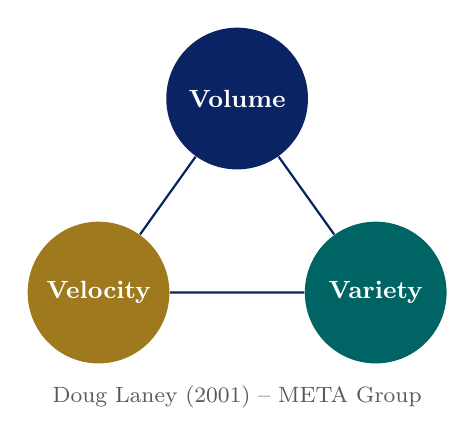
\begin{tikzpicture}[scale=0.88]
        \node[circle, fill=PUNavy, text=white,
              minimum size=1.8cm, font=\bfseries\small,
              align=center] (V) at (2, 2.8) {Volume};
        \node[circle, fill=PUGold!80!black, text=white,
              minimum size=1.8cm, font=\bfseries\small,
              align=center] (Ve) at (0, 0) {Velocity};
        \node[circle, fill=PUTeal, text=white,
              minimum size=1.8cm, font=\bfseries\small,
              align=center] (Va) at (4, 0) {Variety};
        \draw[PUNavy, thick] (V) -- (Ve) -- (Va) -- (V);
        \node[font=\footnotesize, PUGray] at (2, -1.5)
              {Doug Laney (2001) -- META Group};
      \end{tikzpicture}
      \end{center}
      \vspace{6pt}
      \small The 3Vs remain the \textbf{canonical definition} of Big Data, taught in every course from Stanford CS246 to CMU 15-721.
  \end{columns}
\end{frame}
%----------------------------------------------------------------
\begin{frame}{V1\textemdash Volume: The Scale of Data}
  % \begin{columns}[T]
  %   \column{0.56\textwidth}
      \begin{block}{Definition}
        The \textbf{sheer quantity} of data generated, stored, and processed.  Volume is the most intuitive ``big'' in Big Data.
      \end{block}
      \vspace{6pt}
      \textbf{Production-scale examples:}
      \begin{itemize}
        \item \textbf{Facebook / Meta:} 500 TB new data ingested per day
        \item \textbf{Google:} $>$100 PB processed per day (internal, 2023)
        \item \textbf{Walmart:} $>$2.5 PB customer transaction data
        \item \textbf{CERN LHC:} $\approx$15 PB of collision data per year
        \item \textbf{Bangladesh Election Commission:} 110 million NID biometric records
        \item \textbf{bKash:} Millions of micro-transactions per day
      \end{itemize}
      \vspace{4pt}
      \begin{exampleblock}{Textbook Reference}
        \textbf{[SA]} Ch.\,1 $\cdot$ \textbf{[TE]} Ch.\,1 $\cdot$ \textbf{[LRU]} Ch.\,1
      \end{exampleblock}

  %   \column{0.41\textwidth}
  %     \begin{alertblock}{The Engineering Challenge}
  %       How do you store and query 500 TB when the largest single-instance database comfortably handles $\approx$50 TB?
  %     \end{alertblock}
  %     \vspace{6pt}
  %     \begin{block}{Solution Architecture Preview}
  %       \begin{itemize}
  %         \small
  %         \item \textbf{HDFS} (Week 3): Distribute data as 128 MB blocks across a cluster of thousands of commodity nodes
  %         \item \textbf{Replication factor 3}: Every block stored on 3 different nodes
  %         \item \textbf{Horizontal scaling}: Add nodes as data grows linearly\textemdash no downtime
  %         \item \textbf{Cloud object storage}: AWS S3, Google GCS for virtually unlimited scale
  %       \end{itemize}
  %     \end{block}
  % \end{columns}
\end{frame}

\begin{frame}{V1\textemdash Volume: The Scale of Data}
  % \begin{columns}[T]
  %   \column{0.56\textwidth}
  %     \begin{block}{Definition}
  %       The \textbf{sheer quantity} of data generated, stored, and processed.  Volume is the most intuitive ``big'' in Big Data.
  %     \end{block}
  %     \vspace{6pt}
  %     \textbf{Production-scale examples:}
  %     \begin{itemize}
  %       \item \textbf{Facebook / Meta:} 500 TB new data ingested per day
  %       \item \textbf{Google:} $>$100 PB processed per day (internal, 2023)
  %       \item \textbf{Walmart:} $>$2.5 PB customer transaction data
  %       \item \textbf{CERN LHC:} $\approx$15 PB of collision data per year
  %       \item \textbf{Bangladesh Election Commission:} 110 million NID biometric records
  %       \item \textbf{bKash:} Millions of micro-transactions per day
  %     \end{itemize}
  %     \vspace{4pt}
  %     \begin{exampleblock}{Textbook Reference}
  %       \textbf{[SA]} Ch.\,1 $\cdot$ \textbf{[TE]} Ch.\,1 $\cdot$ \textbf{[LRU]} Ch.\,1
  %     \end{exampleblock}

  %   \column{0.41\textwidth}
      \begin{alertblock}{The Engineering Challenge}
        How do you store and query 500 TB when the largest single-instance database comfortably handles $\approx$50 TB?
      \end{alertblock}
      \vspace{6pt}
      \begin{block}{Solution Architecture Preview}
        \begin{itemize}
          \small
          \item \textbf{HDFS} (Week 3): Distribute data as 128 MB blocks across a cluster of thousands of commodity nodes
          \item \textbf{Replication factor 3}: Every block stored on 3 different nodes
          \item \textbf{Horizontal scaling}: Add nodes as data grows linearly\textemdash no downtime
          \item \textbf{Cloud object storage}: AWS S3, Google GCS for virtually unlimited scale
        \end{itemize}
      \end{block}
  % \end{columns}
\end{frame}
%----------------------------------------------------------------
\begin{frame}{V2\textemdash Velocity: The Speed of Data}
  % \begin{columns}[T]
  %   \column{0.56\textwidth}
      \begin{block}{Definition}
        The \textbf{speed} at which data is generated, streamed, and must be processed or acted upon.
      \end{block}
      \vspace{6pt}
      \textbf{High-velocity real-world examples:}
      \begin{itemize}
        \item \textbf{X (Twitter):} 6{,}000 tweets posted per second
        \item \textbf{Visa payment network:} 24{,}000 transactions/second (peak)
        \item \textbf{IoT sensor networks:} 1 billion device readings per hour
        \item \textbf{NYSE / DSE:} Millions of stock quotes per second
        \item \textbf{Pathao (BD):} GPS location ping every 3 s per active driver
        \item \textbf{Mobile banking (bKash):} Real-time fraud scoring in $<$200 ms
      \end{itemize}
      \vspace{4pt}
      \begin{alertblock}{The Engineering Challenge}
        If each DB query takes 50 ms, a system that must handle 6{,}000 events/sec cannot afford serial processing.
      \end{alertblock}

  %   \column{0.41\textwidth}
  %     \begin{block}{Processing Spectrum}
  %       \small
  %       \renewcommand{\arraystretch}{1.25}
  %       \begin{tabular}{lll}
  %         \toprule
  %         \textbf{Mode} & \textbf{Latency} & \textbf{Tool} \\
  %         \midrule
  %         Batch         & Hours    & Hadoop MR \\
  %         Micro-batch   & Seconds  & Spark Streaming \\
  %         Stream        & Millisec & Apache Flink \\
  %         Real-time     & Sub-ms   & Kafka + in-mem \\
  %         \bottomrule
  %       \end{tabular}
  %     \end{block}
  %     \vspace{6pt}
  %     \begin{exampleblock}{Solution Preview}
  %       \begin{itemize}
  %         \small
  %         \item \textbf{Apache Kafka} (Week 8): Distributed log for high-throughput event ingestion
  %         \item \textbf{Spark Streaming} (Week 6): Stateful micro-batch stream processing
  %         \item \textbf{Apache Flink}: True continuous stream processing
  %       \end{itemize}
  %     \end{exampleblock}
  % \end{columns}
\end{frame}
\begin{frame}{V2\textemdash Velocity: The Speed of Data}
  % \begin{columns}[T]
  %   \column{0.56\textwidth}
  %     \begin{block}{Definition}
  %       The \textbf{speed} at which data is generated, streamed, and must be processed or acted upon.
  %     \end{block}
  %     \vspace{6pt}
  %     \textbf{High-velocity real-world examples:}
  %     \begin{itemize}
  %       \item \textbf{X (Twitter):} 6{,}000 tweets posted per second
  %       \item \textbf{Visa payment network:} 24{,}000 transactions/second (peak)
  %       \item \textbf{IoT sensor networks:} 1 billion device readings per hour
  %       \item \textbf{NYSE / DSE:} Millions of stock quotes per second
  %       \item \textbf{Pathao (BD):} GPS location ping every 3 s per active driver
  %       \item \textbf{Mobile banking (bKash):} Real-time fraud scoring in $<$200 ms
  %     \end{itemize}
  %     \vspace{4pt}
  %     \begin{alertblock}{The Engineering Challenge}
  %       If each DB query takes 50 ms, a system that must handle 6{,}000 events/sec cannot afford serial processing.
  %     \end{alertblock}

  %   \column{0.41\textwidth}
      \begin{block}{Processing Spectrum}
        \small
        \renewcommand{\arraystretch}{1.25}
        \begin{tabular}{lll}
          \toprule
          \textbf{Mode} & \textbf{Latency} & \textbf{Tool} \\
          \midrule
          Batch         & Hours    & Hadoop MR \\
          Micro-batch   & Seconds  & Spark Streaming \\
          Stream        & Millisec & Apache Flink \\
          Real-time     & Sub-ms   & Kafka + in-mem \\
          \bottomrule
        \end{tabular}
      \end{block}
      \vspace{6pt}
      \begin{exampleblock}{Solution Preview}
        \begin{itemize}
          \small
          \item \textbf{Apache Kafka} (Week 8): Distributed log for high-throughput event ingestion
          \item \textbf{Spark Streaming} (Week 6): Stateful micro-batch stream processing
          \item \textbf{Apache Flink}: True continuous stream processing
        \end{itemize}
      \end{exampleblock}
  % \end{columns}
\end{frame}
%----------------------------------------------------------------
\begin{frame}{V3\textemdash Variety: The Diversity of Data}
  % \begin{columns}[T]
  %   \column{0.56\textwidth}
      \begin{block}{Definition}
        The \textbf{diversity} of data types, formats, sources, and update cadences that must be jointly ingested, integrated, and analysed.
      \end{block}
      \vspace{6pt}
      \textbf{Sources of variety:}
      \begin{itemize}
        \item Multiple \textbf{formats}: CSV, JSON, XML, Avro, Parquet, DICOM, MP4
        \item Multiple \textbf{sources}: RDBMS, REST APIs, sensors, social media, ERP
        \item Multiple \textbf{languages} and character encodings (UTF-8, UTF-16, Bengali)
        \item Multiple \textbf{update frequencies}: historical snapshots + live streams
        \item Multiple \textbf{semantic meanings}: a ``date'' field could be birth date, event date, or record-entry date\textemdash all different
      \end{itemize}

  %   \column{0.41\textwidth}
  %     \begin{alertblock}{The Engineering Challenge}
  %       How do you JOIN a customer record from MySQL with their social media posts, call-centre audio transcription, and purchase-history CSV, all in one query?
  %     \end{alertblock}
  %     \vspace{6pt}
  %     \begin{exampleblock}{Bangladesh Government Analytics Platform}
  %       Integrating data from 50 district hospitals requires:
  %       \vspace{2pt}
  %       \begin{itemize}
  %         \small
  %         \item MySQL RDBMS tables (structured)
  %         \item Pharmacy sales CSV files (structured)
  %         \item Community health worker XML reports (semi-structured)
  %         \item DGHS REST API JSON feeds (semi-structured)
  %         \item Scanned paper forms via OCR (unstructured $\to$ structured)
  %       \end{itemize}
  %     \end{exampleblock}
  % \end{columns}
\end{frame}

\begin{frame}{V3\textemdash Variety: The Diversity of Data}
  % \begin{columns}[T]
  %   \column{0.56\textwidth}
  %     \begin{block}{Definition}
  %       The \textbf{diversity} of data types, formats, sources, and update cadences that must be jointly ingested, integrated, and analysed.
  %     \end{block}
  %     \vspace{6pt}
  %     \textbf{Sources of variety:}
  %     \begin{itemize}
  %       \item Multiple \textbf{formats}: CSV, JSON, XML, Avro, Parquet, DICOM, MP4
  %       \item Multiple \textbf{sources}: RDBMS, REST APIs, sensors, social media, ERP
  %       \item Multiple \textbf{languages} and character encodings (UTF-8, UTF-16, Bengali)
  %       \item Multiple \textbf{update frequencies}: historical snapshots + live streams
  %       \item Multiple \textbf{semantic meanings}: a ``date'' field could be birth date, event date, or record-entry date\textemdash all different
  %     \end{itemize}

  %   \column{0.41\textwidth}
      \begin{alertblock}{The Engineering Challenge}
        How do you JOIN a customer record from MySQL with their social media posts, call-centre audio transcription, and purchase-history CSV, all in one query?
      \end{alertblock}
      \vspace{6pt}
      \begin{exampleblock}{Bangladesh Government Analytics Platform}
        Integrating data from 50 district hospitals requires:
        \vspace{2pt}
        \begin{itemize}
          \small
          \item MySQL RDBMS tables (structured)
          \item Pharmacy sales CSV files (structured)
          \item Community health worker XML reports (semi-structured)
          \item DGHS REST API JSON feeds (semi-structured)
          \item Scanned paper forms via OCR (unstructured $\to$ structured)
        \end{itemize}
      \end{exampleblock}
  % \end{columns}
\end{frame}
%----------------------------------------------------------------
\begin{frame}{Extended Framework: The 5Vs of Big Data}
  \centering
  \renewcommand{\arraystretch}{1.45}
  \begin{tabular}{p{1.8cm}p{4.5cm}p{5.2cm}}
    \toprule
    \textbf{V} & \textbf{Definition} & \textbf{Real-World Example} \\
    \midrule
    \alert{\textbf{Volume}} &
      Scale of data stored and generated &
      Facebook: 500 TB/day ingested \\

    \alert{\textbf{Velocity}} &
      Speed of generation and required processing &
      Visa: 24{,}000 transactions per second \\

    \alert{\textbf{Variety}} &
      Diversity of formats, types and sources &
      CSV + JSON + DICOM + audio files \\

    \textbf{Veracity} &
      Trustworthiness and accuracy of data &
      GPS signal drift, OCR errors, bot tweets, missing sensor readings \\

    \textbf{Value} &
      Business/societal utility extracted from data &
      Revenue gain, lives saved, fraud prevented \\
    \bottomrule
  \end{tabular}
  % %\vspace{8pt}
  % \begin{alertblock}{Critical Distinction}
  %   The \textbf{original 3Vs} (Laney, 2001) addressed \emph{systems} challenges.  The \textbf{extended 5Vs} (Gartner, 2012) added data \emph{quality} (Veracity) and business \emph{justification} (Value)\textemdash recognising that large, fast, varied data must also be \emph{trustworthy} and \emph{useful}.
  % \end{alertblock}
\end{frame}

\begin{frame}{Extended Framework: The 5Vs of Big Data}
  % \centering
  % \renewcommand{\arraystretch}{1.45}
  % \begin{tabular}{p{1.8cm}p{4.5cm}p{5.2cm}}
  %   \toprule
  %   \textbf{V} & \textbf{Definition} & \textbf{Real-World Example} \\
  %   \midrule
  %   \alert{\textbf{Volume}} &
  %     Scale of data stored and generated &
  %     Facebook: 500 TB/day ingested \\

  %   \alert{\textbf{Velocity}} &
  %     Speed of generation and required processing &
  %     Visa: 24{,}000 transactions per second \\

  %   \alert{\textbf{Variety}} &
  %     Diversity of formats, types and sources &
  %     CSV + JSON + DICOM + audio files \\

  %   \textbf{Veracity} &
  %     Trustworthiness and accuracy of data &
  %     GPS signal drift, OCR errors, bot tweets, missing sensor readings \\

  %   \textbf{Value} &
  %     Business/societal utility extracted from data &
  %     Revenue gain, lives saved, fraud prevented \\
  %   \bottomrule
  % \end{tabular}
  % %\vspace{8pt}
  \begin{alertblock}{Critical Distinction}
    The \textbf{original 3Vs} (Laney, 2001) addressed \emph{systems} challenges.  The \textbf{extended 5Vs} (Gartner, 2012) added data \emph{quality} (Veracity) and business \emph{justification} (Value)\textemdash recognising that large, fast, varied data must also be \emph{trustworthy} and \emph{useful}.
  \end{alertblock}
\end{frame}
%================================================================
\section{Distributed Computing Fundamentals}
%================================================================

\begin{frame}{Scaling Strategies: Vertical vs.\ Horizontal}
  % \begin{columns}[T]
  %   \column{0.48\textwidth}
      \begin{block}{Vertical Scaling (Scale Up)}
        Add more power to \textbf{one machine}: faster CPU, more RAM, larger disks.
        \vspace{4pt}
        \begin{itemize}
          \item Simple\textemdash no distributed-systems complexity
          \item Hard physical ceiling (max RAM $\approx$ 64 TB today)
          \item Single point of failure
          \item \textbf{Exponentially expensive}: a $2\times$ more powerful server often costs $8\times$ more
        \end{itemize}
      \end{block}
      \begin{alertblock}{Traditional RDBMS Approach}
        Oracle Exadata (vertical) can cost \$500{,}000+/year in licences alone.
      \end{alertblock}

  %   \column{0.48\textwidth}
  %     \begin{exampleblock}{Horizontal Scaling (Scale Out)}
  %       Add more \textbf{commodity machines} to the cluster.
  %       \vspace{4pt}
  %       \begin{itemize}
  %         \item Each node is cheap (\$3{,}000--\$8{,}000 commodity server)
  %         \item Near-linear scalability: $2\times$ nodes $\approx$ $2\times$ throughput
  %         \item Fault tolerant: losing one node does not halt the cluster
  %         \item Google's GFS cluster (2003): \textbf{thousands} of commodity PCs, each expected to fail
  %       \end{itemize}
  %     \end{exampleblock}
  %     \vspace{4pt}
  %     \begin{block}{Yahoo! Production Evidence (2008)}
  %       10{,}000 commodity nodes, 5 PB storage\textemdash cheaper than one equivalent mainframe, and far more fault tolerant.
  %     \end{block}
  % \end{columns}
\end{frame}

\begin{frame}{Scaling Strategies: Vertical vs.\ Horizontal}
  % \begin{columns}[T]
  %   \column{0.48\textwidth}
  %     \begin{block}{Vertical Scaling (Scale Up)}
  %       Add more power to \textbf{one machine}: faster CPU, more RAM, larger disks.
  %       \vspace{4pt}
  %       \begin{itemize}
  %         \item Simple\textemdash no distributed-systems complexity
  %         \item Hard physical ceiling (max RAM $\approx$ 64 TB today)
  %         \item Single point of failure
  %         \item \textbf{Exponentially expensive}: a $2\times$ more powerful server often costs $8\times$ more
  %       \end{itemize}
  %     \end{block}
  %     \begin{alertblock}{Traditional RDBMS Approach}
  %       Oracle Exadata (vertical) can cost \$500{,}000+/year in licences alone.
  %     \end{alertblock}

  %   \column{0.48\textwidth}
      \begin{exampleblock}{Horizontal Scaling (Scale Out)}
        Add more \textbf{commodity machines} to the cluster.
        \vspace{4pt}
        \begin{itemize}
          \item Each node is cheap (\$3{,}000--\$8{,}000 commodity server)
          \item Near-linear scalability: $2\times$ nodes $\approx$ $2\times$ throughput
          \item Fault tolerant: losing one node does not halt the cluster
          \item Google's GFS cluster (2003): \textbf{thousands} of commodity PCs, each expected to fail
        \end{itemize}
      \end{exampleblock}
      \vspace{4pt}
      \begin{block}{Yahoo! Production Evidence (2008)}
        10{,}000 commodity nodes, 5 PB storage\textemdash cheaper than one equivalent mainframe, and far more fault tolerant.
      \end{block}
  % \end{columns}
\end{frame}

%----------------------------------------------------------------
\begin{frame}{The CAP Theorem (Brewer, 2000)}
  % \begin{columns}[T]
  %   \column{0.52\textwidth}
      \begin{block}{Theorem Statement (Brewer, PODC 2000; formally proved: Gilbert \& Lynch, 2002)}
        A distributed data system can simultaneously guarantee \textbf{at most two} of:
        \vspace{4pt}
        \begin{itemize}
          \item \textbf{C}onsistency: every read returns the most recent write
          \item \textbf{A}vailability: every request receives a response (not guaranteed to be latest)
          \item \textbf{P}artition tolerance: system operates despite network partitions
        \end{itemize}
      \end{block}
      \vspace{4pt}
      \begin{alertblock}{Practical Implication}
        In any real distributed system, network partitions \emph{will} occur.  P must be tolerated.  Therefore, the design choice is always \textbf{C vs.\ A}.
      \end{alertblock}

  %   \column{0.45\textwidth}
  %     \vspace{4pt}
  %     \begin{center}
  %     \begin{tikzpicture}[scale=0.82]
  %       % Triangle outline
  %       \draw[PUNavy, very thick] (2,3.5) -- (0,0) -- (4,0) -- cycle;
  %       % Corner labels
  %       \node[font=\footnotesize\bfseries, text=PUNavy, align=center] at (2,3.9) {Consistency (C)};
  %       \node[font=\footnotesize\bfseries, text=PUNavy, align=center] at (-1.1,-0.4) {Availability (A)};
  %       \node[font=\footnotesize\bfseries, text=PUNavy, align=center] at (5.1,-0.4) {Partition (P)};
  %       % Edge labels (systems)
  %       \node[font=\scriptsize, align=center, text=PUGold!80!black]
  %             at (1.0, 2.0) {\textbf{CP}\\HBase\\ZooKeeper};
  %       \node[font=\scriptsize, align=center, text=PUTeal]
  %             at (3.0, 2.0) {\textbf{AP}\\Cassandra\\DynamoDB};
  %       \node[font=\scriptsize, align=center]
  %             at (2.0, 0.55) {\textbf{CA}\\MySQL, PostgreSQL\\(no partition)};
  %     \end{tikzpicture}
  %     \end{center}
  %     \vspace{2pt}
  %     \begin{exampleblock}{Big Data Choices}
  %       \small
  %       \textbf{HBase} (CP): used in Hadoop\textemdash strong consistency, sacrifices availability on partition.\\
  %       \textbf{Cassandra} (AP): used by Netflix\textemdash always available, eventual consistency.
  %     \end{exampleblock}
  % \end{columns}
\end{frame}

\begin{frame}{The CAP Theorem (Brewer, 2000)}
  % \begin{columns}[T]
  %   \column{0.52\textwidth}
  %     \begin{block}{Theorem Statement (Brewer, PODC 2000; formally proved: Gilbert \& Lynch, 2002)}
  %       A distributed data system can simultaneously guarantee \textbf{at most two} of:
  %       \vspace{4pt}
  %       \begin{itemize}
  %         \item \textbf{C}onsistency: every read returns the most recent write
  %         \item \textbf{A}vailability: every request receives a response (not guaranteed to be latest)
  %         \item \textbf{P}artition tolerance: system operates despite network partitions
  %       \end{itemize}
  %     \end{block}
  %     \vspace{4pt}
  %     \begin{alertblock}{Practical Implication}
  %       In any real distributed system, network partitions \emph{will} occur.  P must be tolerated.  Therefore, the design choice is always \textbf{C vs.\ A}.
  %     \end{alertblock}

  %   \column{0.45\textwidth}
      \vspace{4pt}
      \begin{center}
      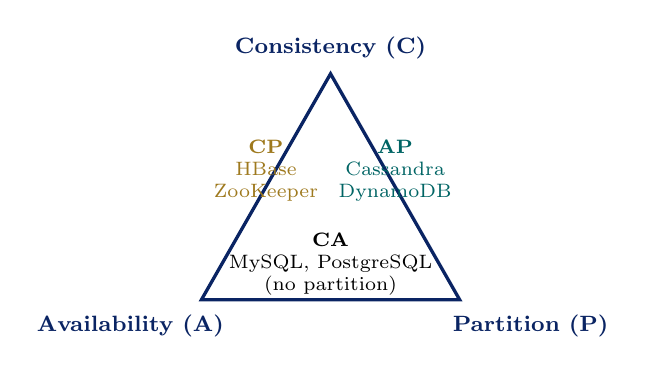
\begin{tikzpicture}[scale=0.82]
        % Triangle outline
        \draw[PUNavy, very thick] (2,3.5) -- (0,0) -- (4,0) -- cycle;
        % Corner labels
        \node[font=\footnotesize\bfseries, text=PUNavy, align=center] at (2,3.9) {Consistency (C)};
        \node[font=\footnotesize\bfseries, text=PUNavy, align=center] at (-1.1,-0.4) {Availability (A)};
        \node[font=\footnotesize\bfseries, text=PUNavy, align=center] at (5.1,-0.4) {Partition (P)};
        % Edge labels (systems)
        \node[font=\scriptsize, align=center, text=PUGold!80!black]
              at (1.0, 2.0) {\textbf{CP}\\HBase\\ZooKeeper};
        \node[font=\scriptsize, align=center, text=PUTeal]
              at (3.0, 2.0) {\textbf{AP}\\Cassandra\\DynamoDB};
        \node[font=\scriptsize, align=center]
              at (2.0, 0.55) {\textbf{CA}\\MySQL, PostgreSQL\\(no partition)};
      \end{tikzpicture}
      \end{center}
      \vspace{2pt}
      \begin{exampleblock}{Big Data Choices}
        \small
        \textbf{HBase} (CP): used in Hadoop\textemdash strong consistency, sacrifices availability on partition.\\
        \textbf{Cassandra} (AP): used by Netflix\textemdash always available, eventual consistency.
      \end{exampleblock}
  % \end{columns}
\end{frame}
%----------------------------------------------------------------
\begin{frame}{Batch vs.\ Stream Processing}
  \centering
  \renewcommand{\arraystretch}{1.4}
  \begin{tabular}{p{2.6cm}p{4.3cm}p{4.3cm}}
    \toprule
    \textbf{Dimension} & \textbf{Batch Processing} & \textbf{Stream Processing} \\
    \midrule
    Data state       & Stored / historical        & In-motion / live \\
    Latency          & Minutes to hours           & Milliseconds to seconds \\
    Throughput       & Very high (optimised for)  & Moderate \\
    Fault recovery   & Re-run the batch           & Exactly-once semantics \\
    Typical use case & Monthly billing, ML training, nightly ETL & Fraud detection, real-time alerts, live dashboards \\
    Technologies     & Hadoop MapReduce, Hive, Spark Batch & Apache Kafka, Spark Streaming, Apache Flink \\
    \textbf{Complexity} & Lower                  & Higher \\
    \bottomrule
  \end{tabular}
  \vspace{8pt}
  \begin{alertblock}{Week 8 Preview: Architectural Choice}
    The \textbf{Lambda architecture} runs both layers in parallel (batch for accuracy + stream for latency).  The \textbf{Kappa architecture} replaces both with a single stream-processing pipeline, eliminating dual code maintenance.
  \end{alertblock}
\end{frame}

% %================================================================
% \section{Ivy League Alignment}
% %================================================================

% \begin{frame}{Stanford CS246: Mining Massive Datasets}
%   \begin{columns}[T]
%     \column{0.56\textwidth}
%       \begin{block}{Course Philosophy (Leskovec, Rajaraman \& Ullman)}
%         \small\textit{``The challenge of big data is not just storage\textemdash it is running algorithms that are fast enough to be useful on datasets that do not fit in the memory of a single machine.  This forces a rethinking of everything.''}\\[4pt]
%         \hfill\textemdash\,\textit{Mining of Massive Datasets}, Preface
%       \end{block}
%       \vspace{6pt}
%       \textbf{Key Benchmark: Sub-Quadratic Requirement}
%       \begin{itemize}
%         \item On $n = 10^{9}$ records, an $O(n^{2})$ algorithm requires $10^{18}$ operations
%         \item At $10^{9}$ ops/second, that is \textbf{31.7 years} of compute time
%         \item Big Data forces every algorithm to target $O(n)$ or $O(n \log n)$
%         \item MapReduce and Spark enforce \textbf{single-pass or logarithmic-pass} processing over data
%       \end{itemize}

%     \column{0.41\textwidth}
%       \begin{exampleblock}{Benchmarks Across Ivy League}
%         \small
%         \begin{itemize}
%           \item \textbf{Stanford CS246}: MapReduce, Spark, LSH, graph mining, recommender systems
%           \item \textbf{Harvard CS265}: Storage systems, query optimisation, indexing at scale
%           \item \textbf{MIT 6.830}: Distributed consistency, transaction models
%           \item \textbf{CMU 15-721}: Modern columnar and in-memory databases
%           \item \textbf{Columbia COMS 4995}: End-to-end big data engineering pipelines
%         \end{itemize}
%       \end{exampleblock}
%       \vspace{4pt}
%       \begin{alertblock}{CSE 4345 Positioning}
%         This course covers the \textbf{foundational stack} (Hadoop, HDFS, MapReduce, Spark, Hive) upon which all of the above advanced courses build.
%       \end{alertblock}
%   \end{columns}
% \end{frame}

%================================================================
\section{Student Assessment Pool}
%================================================================

\begin{frame}{Assessment\textemdash Multiple Choice Questions: Set A \hfill\small\textit{CLO1}}
  \begin{exampleblock}{Instructions}
    Select the single best answer.  Answers are \textbf{bolded} for instructor reference; present without bold to students.
  \end{exampleblock}
  \vspace{8pt}
  \begin{enumerate}[\textbf{Q1.}]
    \item Who first formally proposed the \textbf{3Vs} framework for Big Data?
    \begin{enumerate}[(a)]
      \item Jim Gray \quad
      (b) \textbf{Doug Laney} \quad
      (c) Jeffrey Dean \quad
      (d) Erik Brynjolfsson
    \end{enumerate}
  \end{enumerate}
  \vspace{6pt}
  \begin{enumerate}[\textbf{Q2.}]
    \item Which of the following is an example of \textbf{unstructured data}?
    \begin{enumerate}[(a)]
      \item SQL relational table \quad
      (b) CSV file \quad
      (c) \textbf{MRI scan image} \quad
      (d) JSON API response
    \end{enumerate}
  \end{enumerate}
  \vspace{10pt}
  \begin{alertblock}{Instructor Notes}
    \textbf{Q1:} Students commonly confuse Laney with MapReduce authors (Dean \& Ghemawat).  \textbf{Q2:} JSON (option d) is a common wrong answer\textemdash it is \emph{semi}-structured because it carries key names; an MRI has no schema at all.
  \end{alertblock}
\end{frame}

%----------------------------------------------------------------
\begin{frame}{Assessment\textemdash Multiple Choice Questions: Set B \hfill\small\textit{CLO1}}
  \vspace{6pt}
  \begin{enumerate}[\textbf{Q3.}]
    \item The CAP theorem states that a distributed system cannot simultaneously guarantee more than two of:
    \begin{enumerate}[(a)]
      \item Cost, Availability, Performance
      \item \textbf{Consistency, Availability, Partition Tolerance}
      \item Correctness, Atomicity, Persistence
      \item Concurrency, Accuracy, Partitioning
    \end{enumerate}
  \end{enumerate}
  \vspace{8pt}
  \begin{enumerate}[\textbf{Q4.}]
    \item Which ``V'' of Big Data specifically refers to the \textbf{speed} at which data is generated and must be processed?
    \begin{enumerate}[(a)]
      \item Volume \quad
      (b) Variety \quad
      (c) \textbf{Velocity} \quad
      (d) Veracity
    \end{enumerate}
  \end{enumerate}
  \vspace{10pt}
  \begin{alertblock}{Instructor Notes}
    \textbf{Q3:} All four options are designed to sound plausible\textemdash requires precise recall.  \textbf{Q4:} ``Veracity'' (option d) is the most common wrong answer since it starts with ``Ve-''; students must know the precise definitions of each V.
  \end{alertblock}
\end{frame}

%----------------------------------------------------------------
\begin{frame}{Assessment\textemdash True / False \hfill\small\textit{CLO1}}
  \begin{block}{Instructions}
    State True or False.  Award full marks only if the student provides a \textbf{one-sentence justification}.
  \end{block}
  \vspace{6pt}
  \centering
  \renewcommand{\arraystretch}{1.55}
  \begin{tabular}{p{9.0cm}c}
    \toprule
    \textbf{Statement} & \textbf{Answer} \\
    \midrule
    1.\ \ Structured data accounts for approximately 80\% of all digital data in the world. & \alert{\textbf{False}} \\
    2.\ \ The 3Vs Big Data framework was extended to 5Vs by adding Veracity and Value. & \textbf{True} \\
    3.\ \ Horizontal scaling means adding more RAM and faster CPUs to a single existing server. & \alert{\textbf{False}} \\
    4.\ \ Batch processing is suitable for detecting a stolen credit card being used in real time. & \alert{\textbf{False}} \\
    \bottomrule
  \end{tabular}
  \vspace{8pt}
  \begin{exampleblock}{Justification Model Answers}
    \small \textbf{1:} Unstructured data accounts for $\approx$70--80\%; structured is only $\approx$20\%.  \textbf{3:} That describes \emph{vertical} scaling; horizontal scaling means adding \emph{more machines} to the cluster.  \textbf{4:} Batch incurs latency of minutes to hours; fraud detection requires sub-second \emph{stream} processing.
  \end{exampleblock}
\end{frame}

%----------------------------------------------------------------
\begin{frame}{Assessment\textemdash Descriptive Questions \hfill\small\textit{CLO1}}
  \begin{block}{Instructions}
    Answer each question in \textbf{100--150 words}.  Use specific terminology covered in class.
  \end{block}
  \vspace{10pt}
  \begin{enumerate}[\textbf{D1.}]
    \item Explain the \textbf{3Vs} (and the extended 5Vs) of Big Data, providing one concrete real-world example for \emph{each} dimension.
  \end{enumerate}
  \vspace{8pt}
  \begin{enumerate}[\textbf{D2.}]
    \item Differentiate between \textbf{structured, semi-structured, and unstructured data}.  Provide examples exclusively from the \textbf{healthcare domain in Bangladesh}.
  \end{enumerate}
  \vspace{8pt}
  \begin{enumerate}[\textbf{D3.}]
    \item State and explain the \textbf{CAP theorem}.  Why is it a fundamental constraint for designing distributed Big Data systems?  Give one concrete example of a real system that makes each of the three trade-offs (CA, CP, AP).
  \end{enumerate}
\end{frame}

%----------------------------------------------------------------
\begin{frame}{Assessment\textemdash Analytical Questions \hfill\small\textit{CLO1}}
  \begin{block}{Instructions}
    Answer in \textbf{200--300 words}.  Show step-by-step reasoning.  Partial credit is awarded for correct reasoning even with incomplete conclusions.
  \end{block}
  \vspace{6pt}
  \begin{enumerate}[\textbf{A1.}]
    \item \textbf{5Vs Analysis\textemdash Pathao (Bangladesh ride-sharing):}\\
    Pathao collects a GPS ping every 3 seconds from 500{,}000 active drivers, integrates real-time traffic feeds, surge pricing algorithms, and customer written reviews.
    \begin{itemize}
      \small
      \item Analyse this scenario through \textbf{all 5Vs}.
      \item Which V poses the greatest \textbf{engineering challenge}?  Justify.
      \item What happens to the overall system if Veracity is compromised (GPS signal drifts by 200 m)?
    \end{itemize}
  \end{enumerate}
  \vspace{8pt}
  \begin{enumerate}[\textbf{A2.}]
    \item \textbf{Processing Paradigm Trade-off:}\\
    Compare batch and stream processing for: \textbf{(a)} generating a monthly bank statement, \textbf{(b)} detecting that a stolen bKash mobile account is being drained 10 seconds after theft.  Justify why each scenario demands a different processing model and identify the key engineering trade-offs.
  \end{enumerate}
\end{frame}

%================================================================
\section*{Textbook References}
%================================================================

\begin{frame}{Textbook \& Reading References}
  \begin{block}{Primary Textbooks for Week 1}
    \begin{itemize}
      \item \textbf{[SA]}\ Acharya \& Chellappan. \textit{Big Data and Analytics}, Wiley, 2015.
            \hfill \textbf{Chapter 1}
      \item \textbf{[TE]}\ Erl, Khattak \& Buhler. \textit{Big Data Fundamentals}, Prentice Hall, 2016.
            \hfill \textbf{Chapters 1, 3}
      \item \textbf{[MMS]}\ Mayer-Schönberger \& Cukier. \textit{Big Data: A Revolution}, Houghton Mifflin, 2013.
            \hfill \textbf{Chapter 1}
      \item \textbf{[LRU]}\ Leskovec, Rajaraman \& Ullman. \textit{Mining of Massive Datasets}, 3rd ed., Cambridge, 2020.
            \hfill \textbf{Chapter 1} \\
            {\small\itshape Free PDF: \texttt{mmds.org}}
    \end{itemize}
  \end{block}
  \vspace{6pt}
  \begin{exampleblock}{Supplementary\textemdash Covered in Week 1 Part 2 (Seminal Papers)}
    \small
    \begin{itemize}
      \item Laney, D. (2001). \textit{3D Data Management: Controlling Data Volume, Velocity and Variety}. META Group Research Note. \textbf{[PRIMARY]}
      \item Brewer, E. (2000). \textit{Towards Robust Distributed Systems}. PODC Keynote.
      \item Gilbert \& Lynch (2002). \textit{Brewer's Conjecture and the Feasibility of Consistent Available Partition-Tolerant Web Services}. SIGACT.
      \item Manyika et al. (2011). \textit{Big Data: The Next Frontier for Innovation, Competition, and Productivity}. McKinsey Global Institute. \textbf{[CASE STUDY]}
    \end{itemize}
  \end{exampleblock}
\end{frame}

%----------------------------------------------------------------
\begin{frame}[c]
  \begin{center}
    {\Large\bfseries Questions \& Discussion}\\[10pt]
    {\large Week 1, Part 1 $\;\mid\;$ CSE 4345 Big Data Analytics}\\[8pt]
    \textcolor{PUGray}{\rule{7cm}{0.5pt}}\\[10pt]
    \begin{quote}
    \itshape ``Without data you're just another person with an opinion.''
    \end{quote}
    \hfill\textemdash\,W.\ Edwards Deming
    \vspace{16pt}
    \begin{block}{\centering Next Lecture: Week 1, Part 2}
      \centering
      Seminal Research: Laney (2001) $\cdot$ CAP Theorem Formal Proof\\
      Case Study: McKinsey Global Institute (2011) $\cdot$ Live Data Exercise
    \end{block}
  \end{center}
\end{frame}

%=================================================================
\end{document}
%=================================================================
